\chapter{Função da Forma (Métodos, Funções)}\label{cap:funcoes}


É muito comum ao desenvolver um programa, verificarmos que existem conjuntos de operações muito semelhantes
que são executadas várias vezes, em pontos diferentes do programa. 
Vamos supor que queremos desenvolver um programa que desenhe uma ``cara'' no ecrã:
\begin{center}
	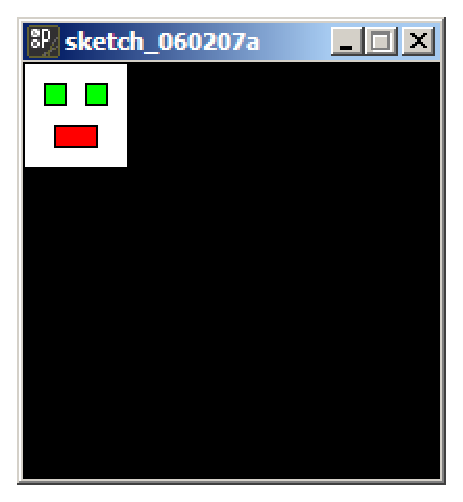
\includegraphics[width=4cm]{images/cara.eps}
\end{center}
\begin{lstlisting}
void setup() {
    size(200, 200);
}


void draw() {
    background(0);
    
    fill(255, 255, 255);     //branco
    rect(0, 0, 50, 50);      //cara
    
    fill(0, 255, 0);         //verde
    rect(10, 10, 10, 10);    //olho esquerdo
    rect(30, 10, 10, 10);    // olho direito
    
    fill(255, 0, 0);         //vermelho
    rect(15, 30, 20, 10);    // boca
}
\end{lstlisting}

Agora, em vez de apenas uma ``cara'', queremos duas:
\begin{center}
	\includegraphics[width=4cm]{images/cara2.eps}
\end{center}
\begin{lstlisting}
void setup() {
    size(200, 200);
}


void draw() {
    background(0);
    
    fill(255, 255, 255);     //branco
    rect(0, 0, 50, 50);      //cara
    
    fill(0, 255, 0);         //verde
    rect(10, 10, 10, 10);    //olho esquerdo
    rect(30, 10, 10, 10);    // olho direito
    
    fill(255, 0, 0);         //vermelho
    rect(15, 30, 20, 10);    // boca

    // segunda cara
    fill(255, 255, 255);     //branco
    rect(100, 0, 50, 50);      //cara
    
    fill(0, 255, 0);         //verde
    rect(110, 10, 10, 10);    //olho esquerdo
    rect(130, 10, 10, 10);    // olho direito
    
    fill(255, 0, 0);         //vermelho
    rect(115, 30, 20, 10);    // boca    
}
\end{lstlisting}
E agora, três:
\begin{center}
	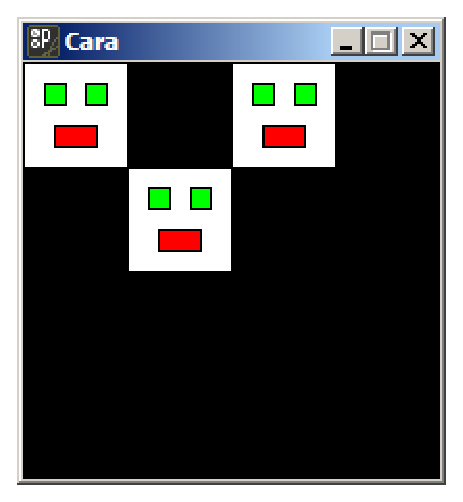
\includegraphics[width=4cm]{images/cara3.eps}
\end{center}
\begin{lstlisting}
void setup() {
    size(200, 200);
}


void draw() {
    background(0);
    
    fill(255, 255, 255);     //branco
    rect(0, 0, 50, 50);      //cara
    
    fill(0, 255, 0);         //verde
    rect(10, 10, 10, 10);    //olho esquerdo
    rect(30, 10, 10, 10);    // olho direito
    
    fill(255, 0, 0);         //vermelho
    rect(15, 30, 20, 10);    // boca
    
    // segunda cara
    fill(255, 255, 255);     //branco
    rect(100, 0, 50, 50);      //cara
    
    fill(0, 255, 0);         //verde
    rect(110, 10, 10, 10);    //olho esquerdo
    rect(130, 10, 10, 10);    // olho direito
    
    fill(255, 0, 0);         //vermelho
    rect(115, 30, 20, 10);    // boca       
    
    // terceira cara
    fill(255, 255, 255);     //branco
    rect(50, 50, 50, 50);      //cara
    
    fill(0, 255, 0);         //verde
    rect(60, 60, 10, 10);    //olho esquerdo
    rect(80, 60, 10, 10);    // olho direito
    
    fill(255, 0, 0);         //vermelho
    rect(65, 80, 20, 10);    // boca           
}

\end{lstlisting}
Se repararem, o código para desenhar as três caras é muito semelhante. Então para quê repeti-lo? A única coisa que muda é a posição onde os rectângulos são desenhados. Para isso podemos utilizar as funções. 

Uma função, ou método%
\footnote{Utilizo as palavras \emph{função} e \emph{método} com o mesmo significado.}%
, é um bloco de código com nome que pode ser executado em qualquer parte do programa. Uma função pode ser chamada%
\footnote{\emph{Chamar} ou \emph{invocar} uma função significa executar o código associado a essa função.}
várias vezes no programa, em pontos distintos.

No caso do exemplo, podemos definir duas variáveis: \texttt{x} e \texttt{y} que indicam onde a ``cara'' irá ser desenhada e criar uma função que utiliza essas variáveis para desenhar apenas uma ``cara'':
\begin{center}
	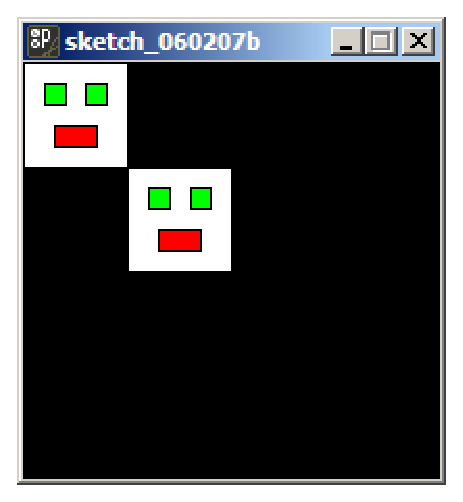
\includegraphics[width=4cm]{images/caraMetodo.eps}
\end{center}
\begin{lstlisting}
int x;
int y;

void setup() {
    size(200, 200);
}

void draw() {
    background(0);
    
    x = 0;
    y = 0;
    desenhaCara();
    
    x = 50;
    y = 50;     
    desenhaCara();  
}

void desenhaCara() {
    fill(255, 255, 255);         //branco
    rect(x, y, 50, 50);          //cara
    
    fill(0, 255, 0);             //verde
    rect(x+10, y+10, 10, 10);    //olho esquerdo
    rect(x+30, y+10, 10, 10);    // olho direito
    
    fill(255, 0, 0);             //vermelho
    rect(x+15, y+30, 20, 10);    // boca       
}
\end{lstlisting}
Neste programa, apenas escrevemos uma vez o código para desenhar a ``cara''. Tivemos de o reescrever ligeiramente de forma a utilizar as variáveis \texttt{x} e \texttt{y} como referência para a posição dos rectângulos, mas nada mais.
Assim, a única coisa que temos de fazer quando quisermos desenhar uma cara é definir a posição e invocar o método \texttt{desenhaCara()}.

Poderiamos, inclusive, utilizar um ciclo para desenhar ``caras''.


\section{Parâmetros}
No exemplo anterior, utilizámos variáveis globais para definir a posição da próxima cara a ser desenhada pela função \texttt{desenhaCara()}. No entanto, seria mais prático se pudessemos ``dizer'' ao programa: \\
-- Desenha uma cara na posição (x, y). Sem recorrer a variáveis globais.

De facto é possível. Uma das características das funções é permitir receber parâmetros que afectam a forma como a função se comporta. Os parâmetros, que não são mais do que valores (qualquer tipo de valor), são passados entre parentesis, a seguir ao nome da função. O parâmetro é identificado pela sua posição relativa, quando definimos a função. Para exemplificar, vamos redefinir a função \texttt{desenhaCara}, de modo a aceitar dois parâmetros: a posição x e a posição y da cara:
\begin{lstlisting}
void desenhaCara(int posicaoX, int posicaoY) {
    fill(255, 255, 255);         //branco
    rect(posicaoX, posicaoY, 50, 50);          //cara
    
    fill(0, 255, 0);             //verde
    rect(posicaoX+10, posicaoY+10, 10, 10);    //olho esquerdo
    rect(posicaoX+30, posicaoY+10, 10, 10);    // olho direito
    
    fill(255, 0, 0);             //vermelho
    rect(posicaoX+15, posicaoY+30, 20, 10);    // boca       
}
\end{lstlisting}
Reparem que colocamos entre parentesis, dois parâmetros: \texttt{posicaoX} e \texttt{posicaoY}. A declaração dos parâmetros é feita de forma semelhande à declaração de variáveis. Temos de indicar qual o tipo e nome da variável. Os vários parâmetros são separados por vírgulas. Dentro da função utilizamos os nomes dos parâmetros%
\footnote{Os parâmetros são, de facto, variáveis locais à função.}
 em vez de os nomes das variáveis globais.
 
Agora só nos falta saber como invocar a nova função. Vamos reescrever o método \texttt{draw()} do exemplo anterior:
\begin{lstlisting}
void draw() {
    background(0);
    
    desenhaCara(0, 0);
    
    desenhaCara(50, 50);  
}
\end{lstlisting}

Agora indicamos a posição da cara directamente na invocação da função. O primeiro valor representa a posição em X e o segundo valor representa a posição em Y. Foi esta a ordem em que definimos os parâmetros na função. 

Obviamente que os valores que passamos na invocação de uma função podem ser o resultado de uma expressão que pode conter variáveis, valores literais ou até outras funções.



\section{Valor de Retorno}

A função que utilizámos nos exemplos anteriores não podia ser utilizada numa expressão como:
\begin{lstlisting}
int x;

x = 3*5 + desenhaCara(20, 20);
\end{lstlisting}
Qual seria o resultado daquela expressão? Para isso precisamos de saber qual o valor a substituir por \texttt{desenhaCara(20, 20)}. Esse valor não existe.

O método \texttt{desenhaCara()} foi declarado como \texttt{void}%
\footnote{A \emph{keyword} \texttt{void} significa \emph{vazio}. Esta \emph{keyword} é utilizada para declarar métodos que não retornam nenhum valor.}%
.
Isto significa que o método não retorna nenhum valor e, por isso, não pode ser usado em expressões de atribuição. Apenas pode ser invocado.

No entanto, há casos em que nos interessa criar funções que fazem determinados cálculos sobre os parâmetros que lhes passamos e que devolvem o resultado desse cálculo. 

Por exemplo vamos supor que precisamos de calcular, para cada equipa do campeonato nacional, a sua pontuação actual.
Para isso precisámos de saber o número de vitórias e empates, uma vez que a pontuação é dada pela fórmula:
 \begin{equation}
pontuacao = vitorias*3 + empates
 \end{equation}
Uma vez que queremos calcular a pontuação de todas as equipas, vamos utilizar vectores para guardar a informação de todas as equipas -- um vector para guardar o número de vitórias, outro para guardar o número de empates e outro para guardar o resultado final do cálculo da pontuação. Vamos inicializar estas estruturas%
\footnote{Pontuação da Primeira Liga 2005/2006, em 13 Fevereiro de 2006. Podemos ver claramente que o Benfica será campeão! ;)}%
:
\begin{lstlisting}
int vitorias[];
int empates[];
int pontuacao[];

void setup() {
    vitorias = new int[18];
    vitorias[0] = 14; // FC Porto
    vitorias[1] = 13; // Sporting
    vitorias[2] = 13; // Benfica 
    vitorias[3] = 12; // Sp. Braga 
    vitorias[4] = 11; // Nacional
    vitorias[5] = 10; // Boavista
    vitorias[6] = 10; // V. Setúbal
    vitorias[7] = 9;  // U. Leiria
    vitorias[8] = 6;  // Marítimo
    vitorias[9] = 7;  // E. Amadora
    vitorias[10] = 6; // Rio Ave
    vitorias[11] = 7; // Académica
    vitorias[12] = 7; // Belenenses
    vitorias[13] = 7; // Paços Ferreira
    vitorias[14] = 7; // Gil Vicente
    vitorias[15] = 6; // Naval
    vitorias[16] = 4; // V. Guimarães
    vitorias[17] = 2; // Penafiel

    empates = new int[18];
    empates[0] = 6;
    empates[1] = 4;
    empates[2] = 4;
    empates[3] = 5;
    empates[4] = 6;
    empates[5] = 8;
    empates[6] = 3;
    empates[7] = 4;
    empates[8] = 9;
    empates[9] = 6;
    empates[10] = 8;
    empates[11] = 5;
    empates[12] = 4;
    empates[13] = 4;
    empates[14] = 3;
    empates[15] = 3;
    empates[16] = 5;
    empates[17] = 5;
}
\end{lstlisting}
Vamos agora calcuar a pontuação de cada equipa, à moda antiga, i.e., sem recorrer a métodos:
\begin{lstlisting}
    pontuacao = new int[18];
    pontuacao[0] = vitorias[0]*2 +empates[0];
    pontuacao[1] = vitorias[1]*2 +empates[1];
    pontuacao[2] = vitorias[2]*2 +empates[2];
    pontuacao[3] = vitorias[3]*2 +empates[3];
    pontuacao[4] = vitorias[4]*2 +empates[4];
    pontuacao[5] = vitorias[5]*2 +empates[5];                
    pontuacao[6] = vitorias[6]*2 +empates[6];
    pontuacao[7] = vitorias[7]*2 +empates[7];
    pontuacao[8] = vitorias[8]*2 +empates[8];
    pontuacao[9] = vitorias[9]*2 +empates[9];
    pontuacao[10] = vitorias[10]*2 +empates[10];
    pontuacao[11] = vitorias[11]*2 +empates[11];                        
    pontuacao[12] = vitorias[12]*2 +empates[12];                        
    pontuacao[13] = vitorias[13]*2 +empates[13];                        
    pontuacao[14] = vitorias[14]*2 +empates[14];                        
    pontuacao[15] = vitorias[15]*2 +empates[15];                        
    pontuacao[16] = vitorias[16]*2 +empates[16];                        
    pontuacao[17] = vitorias[17]*2 +empates[17]; 
\end{lstlisting}
É necessário repetir 18 vezes a expressão para calcular a pontuação! Oops, enganei-me nas contas: multipliquei por 2 em vez de por 3... tenho de corrigir 18 linhas de código:
\begin{lstlisting}
    pontuacao = new int[18];
    pontuacao[0] = vitorias[0]*3 +empates[0];
    pontuacao[1] = vitorias[1]*3 +empates[1];
    pontuacao[2] = vitorias[2]*3 +empates[2];
    pontuacao[3] = vitorias[3]*3 +empates[3];
    pontuacao[4] = vitorias[4]*3 +empates[4];
    pontuacao[5] = vitorias[5]*3 +empates[5];                
    pontuacao[6] = vitorias[6]*3 +empates[6];
    pontuacao[7] = vitorias[7]*3 +empates[7];
    pontuacao[8] = vitorias[8]*3 +empates[8];
    pontuacao[9] = vitorias[9]*3 +empates[9];
    pontuacao[10] = vitorias[10]*3 +empates[10];
    pontuacao[11] = vitorias[11]*3 +empates[11];                        
    pontuacao[12] = vitorias[12]*3 +empates[12];                        
    pontuacao[13] = vitorias[13]*3 +empates[13];                        
    pontuacao[14] = vitorias[14]*3 +empates[14];                        
    pontuacao[15] = vitorias[15]*3 +empates[15];                        
    pontuacao[16] = vitorias[16]*3 +empates[16];                        
    pontuacao[17] = vitorias[17]*3 +empates[17]; 
\end{lstlisting}
Tem de haver uma forma mais simples de fazer isto! E há: os métodos. Vamos criar um método que aceita como parâmetros o número de vitórias e o número de empates e, com base nestes parâmetros, calcula a pontuação:
\begin{lstlisting}
void calculaPontuacao(int vitoria, int empate) {
    int pontos = vitoria*3 + empate;
}
\end{lstlisting}
A única coisa que este método faz, para já, é implementar a expressão da pontuação. Para podermos tirar partido deste método temos de arranjar forma de obter o resultado do cálculo. Para isso temos de redefinir o método, de forma a indicar o tipo de valor que o método devolve. Depois basta utilizar a \emph{keyword} \texttt{return} no final do método para devolver o resultado:
\begin{lstlisting}
int calculaPontuacao(int vitoria, int empate) {
    int pontos = vitoria*3 + empate;
    
    return pontos;
}
\end{lstlisting}
Agora podemos reescrever o nosso programa:
\begin{lstlisting}
    pontuacao = new int[18];
    pontuacao[0] = calculaPontuacao(vitorias[0], empates[0]);
    pontuacao[1] = calculaPontuacao(vitorias[1], empates[1]);
    pontuacao[2] = calculaPontuacao(vitorias[2], empates[2]);
    pontuacao[3] = calculaPontuacao(vitorias[3], empates[3]);
    pontuacao[4] = calculaPontuacao(vitorias[4], empates[4]);
    pontuacao[5] = calculaPontuacao(vitorias[5], empates[5]);                
    pontuacao[6] = calculaPontuacao(vitorias[6], empates[6]);
    pontuacao[7] = calculaPontuacao(vitorias[7], empates[7]);
    pontuacao[8] = calculaPontuacao(vitorias[8], empates[8]);
    pontuacao[9] = calculaPontuacao(vitorias[9], empates[9]);
    pontuacao[10] = calculaPontuacao(vitorias[10], empates[10]);
    pontuacao[11] = calculaPontuacao(vitorias[11], empates[11]);                        
    pontuacao[12] = calculaPontuacao(vitorias[12], empates[12]);                        
    pontuacao[13] = calculaPontuacao(vitorias[13], empates[13]);                        
    pontuacao[14] = calculaPontuacao(vitorias[14], empates[14]);                        
    pontuacao[15] = calculaPontuacao(vitorias[15], empates[15]);                        
    pontuacao[16] = calculaPontuacao(vitorias[16], empates[16]);                       
    pontuacao[17] = calculaPontuacao(vitorias[17], empates[17]);
\end{lstlisting}
Agora, se por acaso nos tivessemos enganado na expressão da pontuação, apenas tinhamos de alterar uma linha de código!
No entanto, ainda temos muitas linhas de código iguais... vamos resolver isso com um ciclo. O código final do nosso programa seria:
\begin{lstlisting}
int vitorias[];
int empates[];
int pontuacao[];

void setup() {
    int i;
    
    vitorias = new int[18];
    vitorias[0] = 14; // FC Porto
    vitorias[1] = 13; // Sporting
    vitorias[2] = 13; // Benfica 
    vitorias[3] = 12; // Sp. Braga 
    vitorias[4] = 11; // Nacional
    vitorias[5] = 10; // Boavista
    vitorias[6] = 10; // V. Setúbal
    vitorias[7] = 9;  // U. Leiria
    vitorias[8] = 6;  // Marítimo
    vitorias[9] = 7;  // E. Amadora
    vitorias[10] = 6; // Rio Ave
    vitorias[11] = 7; // Académica
    vitorias[12] = 7; // Belenenses
    vitorias[13] = 7; // Paços Ferreira
    vitorias[14] = 7; // Gil Vicente
    vitorias[15] = 6; // Naval
    vitorias[16] = 4; // V. Guimarães
    vitorias[17] = 2; // Penafiel

    empates = new int[18];
    empates[0] = 6;
    empates[1] = 4;
    empates[2] = 4;
    empates[3] = 5;
    empates[4] = 6;
    empates[5] = 8;
    empates[6] = 3;
    empates[7] = 4;
    empates[8] = 9;
    empates[9] = 6;
    empates[10] = 8;
    empates[11] = 5;
    empates[12] = 4;
    empates[13] = 4;
    empates[14] = 3;
    empates[15] = 3;
    empates[16] = 5;
    empates[17] = 5;
    
    pontuacao = new int[18];
    for (i = 0; i < 18; i = i + 1) {
        pontuacao[i] = calculaPontuacao(vitorias[i], empates[i]);
    }

}

int calculaPontuacao(int vitoria, int empate) {
    int pontos = vitoria*3 + empate;
    
    return pontos;
}
\end{lstlisting}

O método \texttt{calculaPontuacao()} é diferente dos métodos que criamos anteriormente porque \emph{retorna} um valor. 
Por isso alteramos a declaração do método: em vez de \texttt{void} usámos \texttt{int}, para indicar que o nosso método retorna um valor do tipo \texttt{int}. 
No código do nosso método, a \emph{keyword} \texttt{return} é utilizada para devolver o valor ao código que invocou o nosso método. Quando retornamos um valor, terminamos também a execução do código do nosso método, ou seja, código a seguir ao \texttt{return} nunca é executado. O \texttt{return} pode ser utilizado em qualquer parte do método. Podemos, por exemplo, colocá-lo dentro de um \texttt{if} de forma a retornar valores diferentes consoante a condição...

Os métodos que retornam valores podem ser utilizados em expressões de atribuição. Foi exactamente isso que fizemos no nosso exemplo:
\begin{lstlisting}
    pontuacao[0] = calculaPontuacao(vitorias[0], empates[0]);
\end{lstlisting}
Quando o programa chega a esta linha de código, irá executar o nosso método com os valores dos parâmetros:
\begin{lstlisting}
    pontuacao[0] = calculaPontuacao(14, 6);
\end{lstlisting}
O código do método executa e devolve o valor $14 \times 3+6$ (48):
\begin{lstlisting}
    pontuacao[0] = 48;
\end{lstlisting}

\section{(Quase) Tudo São Métodos}
Grande parte dos programas que escrevemos utilizam métodos definidos pela própria linguagem. Temos vindo a utilizar até aqui métodos como \texttt{rect()}, para desenhar um rectângulo; \texttt{background()} para limpar o fundo do ecrã com uma determinada cor; \texttt{fill()} para mudar a cor de preenchimento do próximo objecto desenhado; etc.
Estes métodos são em tudo semelhantes aos métodos que nós próprios definimos no nosso programa. A única diferença, é que estes foram definidos pela linguagem.

\subsection{Call Me Back... (Callbacks)}
Como vimos, podemos definir os nossos próprios métodos de forma a estruturar melhor o código do nosso programa.
Vimos também, que o Processing possui um conjunto de métodos próprios que podemos utilizar.

No fundo, o que distingue as linguagens de programação é a sua sintaxe e o conjunto de métodos que estão disponíveis ao programador.

Existem alguns métodos que, apesar de sermos nós (programadores) a implementar%
\footnote{\emph{Implementar um método}, é declará-lo e escrever o código que executa dentro desse método.}%
, não somos nós que os invocamos. Estes métodos são métodos pré-definidos pelo Processing, mas que o programador deve re-implementar para tirar partido deles. Por exemplo, o método \texttt{draw()}. Apesar de termos de o declarar e implementar, nunca o invocamos. 

Estes métodos são chamados métodos de \emph{callback}%
\footnote{\emph{Callback}, porque estes métodos são invocados pela própria linguagem em resposta a um evento externo. Ou seja, são \emph{chamados de volta} pela linguagem.}%
.
 
Existem mais métodos de \emph{callback} para além do \texttt{draw()}:
\begin{itemize}
\item \texttt{setup()} -- invocado pelo Processing antes de iniciar o nosso programa. Este método serve para inicializarmos as nossas variáveis. Devemos colocar aqui o código que queremos que execute apenas uma vez, no início do programa.

\item \texttt{draw()} -- invocado periodicamente pelo Processing para actualizar o estado do programa. Neste método devemos colocar o código para desenhar o nosso programa. A frequência com que este método é invocado pelo Processing pode ser controlado.

\item \texttt{keyPressed()} -- invocado pelo Processing quando o utilizador carrega numa tecla do teclado. 

\item \texttt{keyReleased()} -- invocado pelo Processing quando o utilizador larga uma tecla do teclado. 

\item \texttt{mousePressed()} -- invocado pelo Processing quando o utilizador clica num botão do rato.

\item \texttt{mouseMoved()} -- invocado pelo Processing quando o utilizador arrasta o rato.

\item \texttt{mouseDragged()} -- invocado pelo Processing quando o utilizador arrasta o rato mantendo um botão pressionado.

\item \texttt{mouseReleased()} --	invocado pelo Processing quando o utilizador larga um botão do rato.
\end{itemize}

\section{Métodos e Variáveis}
Um programa pode ser visto como um conjunto de caixas espelhadas: se estivermos dentro da caixa conseguimos ver o que se passa cá fora, mas quem está de fora não consegue ver o interior da caixa.
Uma caixa grande representa o programa principal e caixas mais pequenas, dentro da caixa grande, representam os métodos. É útil pensar nestes termos quando queremos entender a visibilidade das variáveis. Uma variável local ao método está ``dentro da caixa pequena'' que representa esse método. Assim, a ``caixa grande'' -- o programa principal -- não consegue aceder às variáveis declaradas no método, mas o método consegue aceder às variáveis do programa principal. De igual modo, um método não consegue ``ver'' as variáveis locais a outro método. A Figura[x] ilustra esta metáfora.
\begin{figure}
	\centering
		\includegraphics{images/cap6-visibilidade-1.eps}
	\caption{Visibilidade de variáveis locais}
	\label{fig:cap6-visibilidade-1}
\end{figure}

\section{Exercícios}
\begin{enumerate}
\item 
Reescreva um dos programas que criou até agora de forma a utilizar métodos.

\item 
Crie um programa que desenha várias mensagens na janela gráfica.

\item
Adapte o exemplo das caras, de modo a utilizar um \texttt{for} para desenhar 100 caras em posições diferentes no ecrã.
\end{enumerate}